\documentclass[a4paper,12pt]{article} % This defines the style of your paper

\usepackage[top = 2.5cm, bottom = 2.5cm, left = 2.5cm, right = 2.5cm]{geometry} 

% Unfortunately, LaTeX has a hard time interpreting German Umlaute. The following two lines and packages should help. If it doesn't work for you please let me know.
\usepackage[T1]{fontenc}
\usepackage[utf8]{inputenc}
\usepackage{pifont}
% \usepackage{ctex}
\usepackage{amsthm, amsmath, amssymb, mathrsfs,mathtools}

% Defining a new theorem style without italics
\newtheoremstyle{nonitalic}% name
  {\topsep}% Space above
  {\topsep}% Space below
  {\upshape}% Body font
  {}% Indent amount
  {\bfseries}% Theorem head font
  {.}% Punctuation after theorem head
  {.5em}% Space after theorem head
  {}% Theorem head spec (can be left empty, meaning ‘normal`)
  
\theoremstyle{nonitalic}
% Define new 'solution' environment
\newtheorem{innercustomsol}{Solution}
\newenvironment{solution}[1]
  {\renewcommand\theinnercustomsol{#1}\innercustomsol}
  {\endinnercustomsol}

% Custom counter for the solutions
\newcounter{solutionctr}
\renewcommand{\thesolutionctr}{(\alph{solutionctr})}

% Environment for auto-numbering with custom format
\newenvironment{autosolution}
  {\stepcounter{solutionctr}\begin{solution}{\thesolutionctr}}
  {\end{solution}}


\newtheorem{problem}{Problem}
\usepackage{color}

% The following two packages - multirow and booktabs - are needed to create nice looking tables.
\usepackage{multirow} % Multirow is for tables with multiple rows within one cell.
\usepackage{booktabs} % For even nicer tables.

% As we usually want to include some plots (.pdf files) we need a package for that.
\usepackage{graphicx} 
\usepackage{subfigure}


% The default setting of LaTeX is to indent new paragraphs. This is useful for articles. But not really nice for homework problem sets. The following command sets the indent to 0.
\usepackage{setspace}
\setlength{\parindent}{0in}
\usepackage{longtable}

% Package to place figures where you want them.
\usepackage{float}

% The fancyhdr package let's us create nice headers.
\usepackage{fancyhdr}

\usepackage{fancyvrb}

%Code environment 
\usepackage{listings} % Required for insertion of code
\usepackage{xcolor} % Required for custom colors

% Define colors for code listing
\definecolor{codegreen}{rgb}{0,0.6,0}
\definecolor{codegray}{rgb}{0.5,0.5,0.5}
\definecolor{codepurple}{rgb}{0.58,0,0.82}
\definecolor{backcolour}{rgb}{0.95,0.95,0.92}

% Code listing style named "mystyle"
\lstdefinestyle{mystyle}{
    backgroundcolor=\color{backcolour},   
    commentstyle=\color{codegreen},
    keywordstyle=\color{magenta},
    numberstyle=\tiny\color{codegray},
    stringstyle=\color{codepurple},
    basicstyle=\ttfamily\footnotesize, % Change to serif font
    breakatwhitespace=false,         
    breaklines=true,                 
    captionpos=b,                    
    keepspaces=true,                 
    numbers=left,                    
    numbersep=5pt,                  
    showspaces=false,                
    showstringspaces=false,
    showtabs=false,                  
    tabsize=2
}

\lstset{style=mystyle}

%%%%%%%%%%%%%%%%%%%%%%%%%%%%%%%%%%%%%%%%%%%%%%%%
% 3. Header (and Footer)
%%%%%%%%%%%%%%%%%%%%%%%%%%%%%%%%%%%%%%%%%%%%%%%%

% To make our document nice we want a header and number the pages in the footer.

\pagestyle{fancy} % With this command we can customize the header style.

\fancyhf{} % This makes sure we do not have other information in our header or footer.

\lhead{\footnotesize EI035 Econometrics II}% \lhead puts text in the top left corner. \footnotesize sets our font to a smaller size.

%\rhead works just like \lhead (you can also use \chead)
\rhead{\footnotesize Jingle Fu} %<---- Fill in your lastnames.

% Similar commands work for the footer (\lfoot, \cfoot and \rfoot).
% We want to put our page number in the center.
\cfoot{\footnotesize \thepage}
\IfFileExists{upquote.sty}{\usepackage{upquote}}{}
\begin{document}


\thispagestyle{empty} % This command disables the header on the first page. 

\begin{tabular}{p{15.5cm}} % This is a simple tabular environment to align your text nicely 
{\large \bf EI035 Econometrics II} \\
The Graduate Institute, Spring 2025, Marko Mlikota\\
\hline % \hline produces horizontal lines.
\\
\end{tabular} % Our tabular environment ends here.

\vspace*{0.3cm} % Now we want to add some vertical space in between the line and our title.

\begin{center} % Everything within the center environment is centered.
	{\Large \bf PS1 Solutions} % <---- Don't forget to put in the right number
	\vspace{2mm}
	
        % YOUR NAMES GO HERE
	{\bf Jingle Fu} % <---- Fill in your names here!
		
\end{center}  

\vspace{0.4cm}
\setstretch{1.2}

\begin{autosolution}
\ 

\begin{lstlisting}[language=R]
set.seed(2025)
n <- 100
u_i <- rnorm(n, mean = 0, sd = sqrt(5))
g_i <- rgamma(n, shape = 2, scale = 2)
r_i <- rbinom(n, size = 1, prob = 0.5)
x_star_i <- numeric(n)

for (i in 1:n) {
if (r_i[i] == 1) {
x_star_i[i] <- rgamma(1, shape = 3, scale = 1)
  } else {
    x_star_i[i] <- rgamma(1, shape = 7, scale = 1)
  }
}

beta_0 <- 400
beta_1 <- 5
beta_2 <- 200
beta_3 <- 10

y_i <- beta_0 + beta_1 * x_star_i + beta_2 * r_i + beta_3 * g_i + u_i

n_i <- rnorm(n, mean = 10, sd = sqrt(3))
b_i <- rnorm(n, mean = 5 + sqrt(x_star_i), sd = sqrt(3))

data <- data.frame(
    y = y_i,
    x_star = x_star_i,
    r = r_i,
    g = g_i,
    n = n_i,
    b = b_i
  )
\end{lstlisting}
\end{autosolution}


\begin{autosolution}
\ 

We consider the true model:
\[
y_i = \beta_0 + \beta_1 x_i^* + \beta_2 r_i + \beta_3 g_i + u_i,
\]
with the following Data Generating Process (DGP):
\begin{itemize}
    \item $u_i \sim N(0,5)$.
    \item $g_i \sim \Gamma(2,2)$, so that 
    \[
    \mathbb{E}[g_i]=\frac{2}{2}=1,\quad \mathbb{V}[g_i]= 2 \times 2^2= 8.
    \]
    \item $r_i \in \{0,1\}$ with $P(r_i=1)=0.5$.
    \item Conditionally on $r_i$, the fertilizer variable $x_i^*$ is distributed as:
    \begin{itemize}
        \item If $r_i=1$: $x_i^* \sim \Gamma(3,1)$, so that 
        \[
        \mathbb{E}[x_i^*\mid r_i=1]=3,\quad \mathbb{V}[x_i^*\mid r_i=1]=3.
        \]
        \item If $r_i=0$: $x_i^* \sim \Gamma(7,1)$, so that 
        \[
        \mathbb{E}[x_i^*\mid r_i=0]=7,\quad \mathbb{V}[x_i^*\mid r_i=0]=7.
        \]
    \end{itemize}
\end{itemize}

By the law of total expectation, we have:
\[
\mathbb{E}[x_i^*]=0.5\cdot 3+0.5\cdot 7=5.
\]
Similarly, by the law of total variance:
\[
\mathbb{V}[x_i^*]=\mathbb{E}\left[\mathbb{V}[x_i^*\mid r_i]\right]+\mathbb{V}\left(\mathbb{E}[x_i^*\mid r_i]\right)
=0.5\cdot 3+0.5\cdot 7+0.5\Big[(3-5)^2+(7-5)^2\Big]=5+4=9.
\]

% \paragraph{Calculation of $\operatorname{Cov}(x_i^*, g_i)$}

% We have
% \[
% \operatorname{Cov}(x_i^*, g_i)=\mathbb{E}[x_i^*g_i]-\mathbb{E}[x_i^*]\,\mathbb{E}[g_i].
% \]
% Since $\mathbb{E}[x_i^*]=5$ and $\mathbb{E}[g_i]=1$, it remains to compute $\mathbb{E}[x_i^*g_i]$. Conditioning on $r_i$,
% \[
% \mathbb{E}[x_i^*g_i]=E\left[\mathbb{E}[x_i^*g_i\mid r_i]\right]=0.5\,\mathbb{E}[x_i^*g_i\mid r_i=1]+0.5\,\mathbb{E}[x_i^*g_i\mid r_i=0].
% \]
% For each group we write:
% \[
% \mathbb{E}[x_i^*g_i\mid r_i=i]=\mathbb{E}[x_i^*\mid r_i=i]\mathbb{E}[g_i\mid r_i=i]+\operatorname{Cov}(x_i^*,g_i\mid r_i=i),\quad i=0,1.
% \]
% Since the DGP does not explicitly state a dependence between $x_i^*$ and $g_i$, we denote their conditional covariance by
% \[
% \operatorname{Cov}(x_i^*,g_i\mid r_i=i)=\rho_i\sqrt{\mathbb{V}[x_i^*\mid r_i=i]\mathbb{V}[g_i]},\quad i=0,1,
% \]
% with $\rho_i$ being the (conditional) correlation. Thus, for $r_i=1$:
% \[
% \mathbb{E}[x_i^*g_i\mid r_i=1]=3\cdot 1+\rho_1\sqrt{3\cdot 0.5}=3+\rho_1\sqrt{1.5},
% \]
% and for $r_i=0$:
% \[
% \mathbb{E}[x_i^*g_i\mid r_i=0]=7\cdot 1+\rho_0\sqrt{7\cdot 0.5}=7+\rho_0\sqrt{3.5}.
% \]
% Averaging, we obtain:
% \[
% \mathbb{E}[x_i^*g_i]=5+\frac{1}{2}\left(\rho_1\sqrt{1.5}+\rho_0\sqrt{3.5}\right).
% \]
% Therefore,
% \[
% \operatorname{Cov}(x_i^*, g_i)=\frac{1}{2}\left(\rho_1\sqrt{1.5}+\rho_0\sqrt{3.5}\right).
% \]

\textbf{Regression 1:} $y_i = \beta_0 + \beta_1 x^*_i + \text{error}_i$

The working regression is
\[
y_i=\beta_0+\beta_1x_i^*+\varepsilon_i,\quad\text{with}\quad \varepsilon_i=\beta_2r_i+\beta_3g_i+u_i.
\]
The OLS estimator for $\beta_1$ is given by
\[
\hat{\beta}_1=\beta_1+\frac{\operatorname{Cov}\left(x_i^*,\,\beta_2r_i+\beta_3g_i\right)}{\mathbb{V}[x_i^*]}.
\]
By linearity,
\[
\operatorname{Cov}\left(x_i^*,\,\beta_2r_i+\beta_3g_i\right)=\beta_2\,\operatorname{Cov}(x_i^*,r_i)+\beta_3\,\operatorname{Cov}(x_i^*,g_i).
\]

\paragraph{Calculation of $\operatorname{Cov}(x_i^*,r_i)$:} 
\[
\operatorname{Cov}(x_i^*,r_i)=\mathbb{E}[x_i^*r_i]-\mathbb{E}[x_i^*]\,\mathbb{E}[r_i].
\]
Since
\[
\mathbb{E}[x_i^*r_i]=P(r_i=1)\mathbb{E}[x_i^*\mid r_i=1]+P(r_i=0)\cdot 0=0.5\cdot 3=1.5,
\]
and $\mathbb{E}[r_i]=0.5$, it follows that
\[
\operatorname{Cov}(x_i^*,r_i)=1.5-5\cdot 0.5=1.5-2.5=-1.
\]

\paragraph{Calculation of $\operatorname{Cov}(x_i^*,g_i)$:}

From the construction of $g_i$, we have $\operatorname{Cov}(x_i^*,g_i) = 0.$

Thus, the probability limit of $\hat{\beta}_1$ is:
\[
\operatorname*{plim}\hat{\beta}_1=\beta_1+\frac{\beta_2(-1)+\beta_3 (0)}{9} = \beta_1 - \frac{\beta_2}{9} \approx -17.22.
\]

Our simulated result replrts a mean of -16.98, with a standard error of 2.5386, which is close to our theoretical expectation, 
but far from the true value of 5.
% This is a misspecified model due to omitted variables. The OLS estimator for $\beta_1$ in this regression is:
% \[
% \hat{\beta}_1^{(1)} = \frac{\text{Cov}(y_i, x^*_i)}{\text{Var}(x^*_i)}
% \]
% Substituting the true model:
% \[
% \hat{\beta}_1^{(1)} = \frac{\text{Cov}(\beta_0 + \beta_1 x^*_i + \beta_2 r_i + \beta_3 g_i + u_i,\, x^*_i)}{\text{Var}(x^*_i)}
% \]
% Since $\text{Cov}(x^*_i, \beta_0) = 0$ and $\text{Cov}(x^*_i, u_i) = 0$ by assumption:
% \[
% \hat{\beta}_1^{(1)} = \beta_1 + \beta_2 \frac{\text{Cov}(r_i, x^*_i)}{\text{Var}(x^*_i)} + \beta_3 \frac{\text{Cov}(g_i, x^*_i)}{\text{Var}(x^*_i)}
% \]
% According to the DGP, fertilizer application $x^*_i$ depends on land quality $r_i$:
% \begin{itemize}
%     \item When $r_i = 1$: $x^*_i \sim \Gamma(3, 1)$
%     \item When $r_i = 0$: $x^*_i \sim \Gamma(7, 1)$
% \end{itemize}
% This means $\text{Cov}(r_i, x^*_i) \neq 0$. Specifically, since $E[x^*_i \mid r_i=1] = 3$ and $E[x^*_i \mid r_i=0] = 7$, we have a negative covariance (higher $r_i$ corresponds to lower $x^*_i$ on average).

% If we assume $g_i$ and $x^*_i$ are independent, then $\text{Cov}(g_i, x^*_i) = 0$. However, there might be an indirect relationship through $r_i$.

% Therefore, we expect:
% \[
% E[\hat{\beta}_1^{(1)}] = \beta_1 + \beta_2 \frac{\text{Cov}(r_i, x^*_i)}{\text{Var}(x^*_i)} \neq \beta_1
% \]
% Since $\beta_2 = 200$ and $\text{Cov}(r_i, x^*_i)$ is likely negative, we expect $\hat{\beta}_1^{(1)}$ to be biased downward from the true value of 5.

\begin{lstlisting}[language=R]

\end{lstlisting}

\textbf{Regression 2:} $y_i = \beta_0 + \beta_1 x^*_i + \beta_2 r_i + \text{error}_i$

Now the regression is:
\[
y_i=\beta_0+\beta_1x_i^*+\beta_2r_i+\varepsilon_i,\quad\text{with}\quad \varepsilon_i=\beta_3g_i+u_i.
\]
By the Frisch--Waugh--Lovell theorem, we partial out $r_i$ from $x_i^*$. Define the residual:
\[
\tilde{x}_i=x_i^*-\mathbb{E}[x_i^*\mid r_i],
\]
with
\[
\mathbb{E}[x_i^*\mid r_i]=
\begin{cases}
3,& r_i=1,\\[1mm]
7,& r_i=0.
\end{cases}
\]
Then the OLS estimator becomes:
\[
\hat{\beta}_1=\beta_1+\frac{\operatorname{Cov}\left(\tilde{x}_i,\beta_3g_i\right)}{\mathbb{V}[\tilde{x}_i]}
=\beta_1+\beta_3\,\frac{\operatorname{Cov}(\tilde{x}_i,g_i)}{\mathbb{V}[\tilde{x}_i]}.
\]
Assuming that $\mathbb{E}[g_i\mid r_i]=\mathbb{E}[g_i]=1$, note that
\[
\operatorname{Cov}(\tilde{x}_i,g_i)=\operatorname{Cov}(x_i^*,g_i)-\operatorname{Cov}(\mathbb{E}[x_i^*\mid r_i],g_i).
\]
A brief calculation shows:
\[
\operatorname{Cov}(\mathbb{E}[x_i^*\mid r_i],g_i)=0.5\left[3\cdot 1+7\cdot 1\right]-\mathbb{E}[x_i^*]\mathbb{E}[g_i]
=5-5=0.
\]
Also,
\[\operatorname{Cov}(x_i^*, g_i) = 0\]
% \[
% \mathbb{V}[\tilde{x}_i]=E\left[\mathbb{V}[x_i^*\mid r_i]\right]
% =0.5\cdot 3+0.5\cdot 7=5.
% \]
Thus, the probability limit is:
\[
\operatorname*{plim}\hat{\beta}_1^{(2)}=\beta_1.
\]
Its variance is given by 
\[ 
\sigma_{\epsilon}^{2} = \mathbb{V}[\beta_3 g_i + u_i] = \beta_3^2 \mathbb{V}[g_i] + 5.
\]

Our simulated result reports a mean of 4.3648, with a standard error of 1.2873, which is closer to the true value and less volatile than regression (1).
% That is, the bias in Regression 2 is:
% \[
% \text{Bias}^{(2)}=\frac{\beta_3\,\left(\rho_1\sqrt{1.5}+\rho_0\sqrt{3.5}\right)}{10}.
% \]
% The asymptotic variance is:
% \[
% \mathbb{V}[\hat{\beta}_1]\approx\frac{1}{n}\,\frac{\mathbb{V}[\beta_3g_i+u_i]}{5}.
% \]
% This regression includes $r_i$ but omits $g_i$. The OLS estimator for $\beta_1$ can be derived as:
% \[
% \hat{\beta}_1^{(2)} = \beta_1 + \beta_3 \frac{\text{Cov}(g_i, x^*_i \mid \text{controlling for } r_i)}{\text{Var}(x^*_i \mid \text{controlling for } r_i)}
% \]
% If $g_i$ is independent of $x^*_i$ after controlling for $r_i$, then $E[\hat{\beta}_1^{(2)}] = \beta_1$. However, if there's remaining correlation, there will still be some bias.

\begin{lstlisting}[language=R]

\end{lstlisting}

\textbf{Regression 3:} $y_i = \beta_0 + \beta_1 x^*_i + \beta_2 r_i + \beta_3 g_i + \text{error}_i$

Here the regression exactly matches the true DGP:
\[
y_i=\beta_0+\beta_1x_i^*+\beta_2r_i+\beta_3g_i+u_i.
\]
Under the exogeneity assumption $\mathbb{E}[u_i\mid x_i^*,r_i,g_i]=0$, the OLS estimator for $\beta_1$ is \textbf{consistent}:
\[
\operatorname*{plim}\hat{\beta}_1^{(3)}=\beta_1.
\]
Its finite-sample variance is given by the standard OLS formula:
\[
\mathbb{V}[\hat{\beta}_1^{(3)}]=\sigma_{\epsilon}^2\left[(X'X)^{-1}\right]_{11},
\]
where the design matrix $X$ includes the moments and cross-moments of $x_i^*$, $r_i$, and $g_i$.

The simulated result reports a mean of 5.0395, with a standard error of 0.0957, which is almost the true value.
% This regression is correctly specified according to the DGP. Therefore:
% \[
% E[\hat{\beta}_1^{(3)}] = \beta_1 = 5
% \]

\begin{lstlisting}[language=R]

\end{lstlisting}

\textbf{Regression 4:} $y_i = \beta_0 + \beta_1 x^*_i + \beta_2 r_i + \beta_4 n_i + \text{error}_i$

Since $n_i\sim N(10,3)$ is generated independently of $x_i^*$, $r_i$, $g_i$, and $u_i$, 
it is an \emph{irrelevant regressor}. 
Under the standard OLS assumptions, 
the inclusion of an irrelevant regressor does not 
cause bias in the estimated coefficient of $x_i^*$:
\[
\operatorname*{plim}\hat{\beta}_1^{(4)} = \beta_1.
\]
However, its inclusion may increase the finite-sample variance of $\hat{\beta}_1$. 
In particular, the variance formula now becomes
\[
\mathbb{V}[\hat{\beta}_1^{(4)}] = \sigma_{\epsilon}^2\left[(X'X)^{-1}\right]_{11},
\]
where the design matrix $X$ now includes the column corresponding to $n_i$. 
If $n_i$ is only weakly correlated with $x_i^*$, 
then the increase in variance is modest. 
In summary, \textbf{Regression 4} yields a consistent estimator for $\beta_1$, with no additional bias but possibly a slight inflation in variance.

The simulated result reports a mean of 4.4641, with a standard error of 1.3123, which satisfies our expectation.
This is because the model introduces an uncorrelated variable $n_i$ that does not affect the estimation of $\beta_1$, 
but reduced the degree of freedom in the model. So, it's variance is higher than regression (2).

\begin{lstlisting}[language=R]

\end{lstlisting}

\textbf{Regression 5:} $y_i = \beta_0 + \beta_1 x^*_i + \beta_2 r_i + \beta_4 b_i + \text{error}_i$

Here,
\[
b_i \sim N\left(5+\sqrt{x_i^*},\,3\right),
\]
so that $b_i$ is a non-linear function of $x_i^*$. 
This implies that $b_i$ is correlated with $x_i^*$. 
In particular, since
\[
\mathbb{E}[b_i\mid x_i^*] = 5 + \sqrt{x_i^*},
\]
we have
\[
\operatorname{Cov}(x_i^*, b_i) \neq 0.
\]
The inclusion of $b_i$ does not cause endogeneity provided that 
\[
\mathbb{E}[u_i \mid x_i^*, r_i, g_i, b_i] = 0.
\]
Thus, by the Frisch--Waugh--Lovell theorem, 
the coefficient $\beta_1$ is still identified and
\[
\operatorname*{plim}\hat{\beta}_1^{(5)} = \beta_1.
\]

However, the strong correlation between $x_i^*$ and $b_i$ increases multicollinearity. 
To see this more formally, consider the variance of $\hat{\beta}_1$ in a multiple regression:
\[
\mathbb{V}[\hat{\beta}_1^{(5)}] = \sigma_{\epsilon}^2 \left[(X'X)^{-1}\right]_{11}.
\]
When $x_i^*$ is highly collinear with $b_i$, 
the effective variation in $x_i^*$ 
(after partialling out the effect of $b_i$ along with $r_i$ and $g_i$) 
is reduced. 
Denote by $R^2_{x,b}$ the coefficient of determination from 
regressing $x_i^*$ on the other regressors (including $b_i$). 
Then, the variance inflation factor (VIF) for $\hat{\beta}_1$ is given by
\[
\text{VIF} = \frac{1}{1-R^2_{x,b}}.
\]
Thus, the asymptotic variance becomes
\[
\mathbb{V}[\hat{\beta}_1^{(5)}] \approx \frac{\sigma_{\epsilon}^2}{n\,\mathbb{V}[x_i^*]}\cdot \frac{1}{1-R^2_{x,b}},
\]
which is larger than that in Regression 3. 
In summary, while \textbf{Regression 5} still provides a consistent estimate of $\beta_1$, 
the estimator's variance is inflated due to the high collinearity between $x_i^*$ and $b_i$.

The simulated result reports a mean of 4.5369, with a standard error of 1.3026, which estimated $\beta$ better than regression (4), but still deviates from the true value.
Also, it's variance is higher than regression (2)

\begin{lstlisting}[language=R]
reg1 <- lm(y ~ x_star, data = data)
summary_reg1 <- summary(reg1)

reg2 <- lm(y ~ x_star + r, data = data)
summary_reg2 <- summary(reg2)

reg3 <- lm(y ~ x_star + r + g, data = data)
summary_reg3 <- summary(reg3)

reg4 <- lm(y ~ x_star + r + n, data = data)
summary_reg4 <- summary(reg4)

reg5 <- lm(y ~ x_star + r + b, data = data)
summary_reg5 <- summary(reg5)

extract_results <- function(reg_summary, reg_name) {
    beta1_estimate <- reg_summary$coefficients["x_star", "Estimate"]
    beta1_se <- reg_summary$coefficients["x_star", "Std. Error"]
    beta1_true <- 5
    
    cat(paste0("\n", reg_name, ":\n"))
    cat(paste0("Estimated beta_1: ", round(beta1_estimate, 4), "\n"))
    cat(paste0("True beta_1: ", beta1_true, "\n"))
    cat(paste0("Standard Error: ", round(beta1_se, 4), "\n"))
    cat(paste0("Difference from true value: ", round(beta1_estimate - beta1_true, 4), "\n"))
    cat(paste0("Adjusted R_2: ", round(reg_summary$adj.r.squared, 4), "\n"))
}

extract_results(summary_reg1, "Regression 1 (y ~ x_star)")
extract_results(summary_reg2, "Regression 2 (y ~ x_star + r)")
extract_results(summary_reg3, "Regression 3 (y ~ x_star + r + g)")
extract_results(summary_reg4, "Regression 4 (y ~ x_star + r + n)")
extract_results(summary_reg5, "Regression 5 (y ~ x_star + r + b)")
\end{lstlisting}

\begin{table}[htbp!]

\caption{Regression Results for Question (b)}
\centering
\begin{tabular}[t]{lrrrr}
\toprule
Regression & $\hat{\beta}_1$ & SE & Difference & Adjusted $R^2$\\
\midrule
y \textasciitilde{} $x^*$ & -16.9809 & 2.5386 & -21.9809 & 0.3065\\
y \textasciitilde{} $x^* + r$ & 4.3648 & 1.2873 & -0.6352 & 0.9029\\
y \textasciitilde{} $x^* + r + g$ & 5.0395 & 0.0957 & 0.0395 & 0.9995\\
y \textasciitilde{} $x^* + r + n$ & 4.4641 & 1.3123 & -0.5359 & 0.9021\\
y \textasciitilde{} $x^* + r + b$ & 4.5369 & 1.3026 & -0.4631 & 0.9027\\
\bottomrule
\end{tabular}
\end{table}
%% Table saved to b.tex


\end{autosolution}


\begin{autosolution}
\ 

From a theoretical perspective, the Monte Carlo simulation allows us to empirically approximate the sampling distribution of each estimator. The histograms should confirm our theoretical derivations:
\begin{enumerate}
    \item $\hat{\beta}_1^{(1)}$ should show a systematic bias from the true value of 5.
    \item $\hat{\beta}_1^{(2)}$ might show a smaller bias if there's still correlation between $g_i$ and $x^*_i$ after controlling for $r_i$.
    \item $\hat{\beta}_1^{(3)}$, $\hat{\beta}_1^{(4)}$, and $\hat{\beta}_1^{(5)}$ should be centered around 5, but with increasing variance.
\end{enumerate}

\begin{figure}[H]
  \centering
  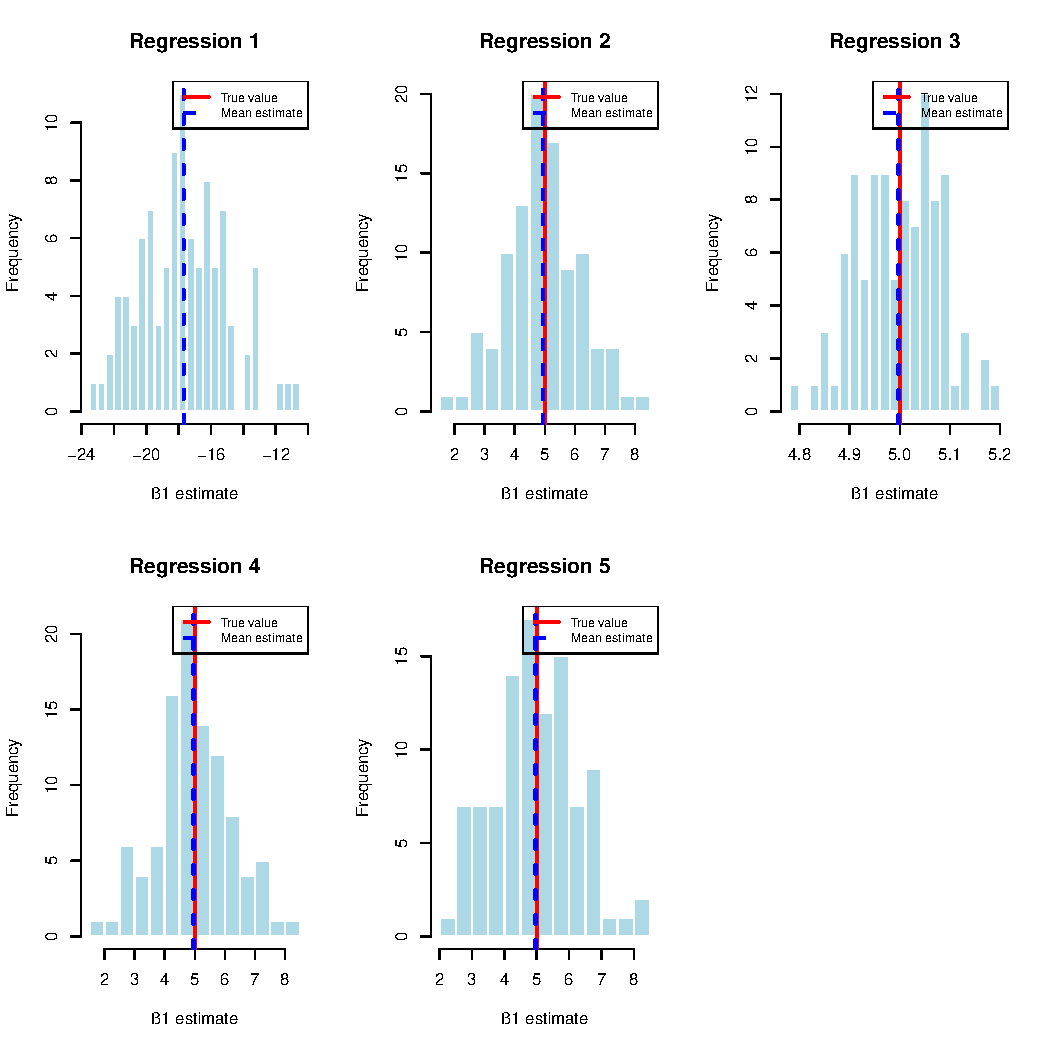
\includegraphics[width=\textwidth]{Q(c).pdf}
  \label{fig:monte_carlo_results}
\end{figure}

\begin{lstlisting}[language=R]
set.seed(2025)
M <- 100
n <- 100

beta1_estimates <- matrix(NA, nrow = M, ncol = 5)
colnames(beta1_estimates) <- c("Reg1", "Reg2", "Reg3", "Reg4", "Reg5")

for (m in 1:M) {
  u_i <- rnorm(n, mean = 0, sd = sqrt(5))
  g_i <- rgamma(n, shape = 2, scale = 2)
  r_i <- rbinom(n, size = 1, prob = 0.5)
    
  x_star_i <- numeric(n)
  for (i in 1:n) {
    if (r_i[i] == 1) {
      x_star_i[i] <- rgamma(1, shape = 3, scale = 1)
    } else {
      x_star_i[i] <- rgamma(1, shape = 7, scale = 1)
    }
  }
    
  beta_0 <- 400
  beta_1 <- 5
  beta_2 <- 200
  beta_3 <- 10
    
  y_i <- beta_0 + beta_1 * x_star_i + beta_2 * r_i + beta_3 * g_i + u_i
    
  n_i <- rnorm(n, mean = 10, sd = sqrt(3))
  b_i <- rnorm(n, mean = 5 + sqrt(x_star_i), sd = sqrt(3))
    
  data <- data.frame(
    y = y_i,
    x_star = x_star_i,
    r = r_i,
    g = g_i,
    n = n_i,
    b = b_i
  )
  
  reg1 <- lm(y ~ x_star, data = data)
  reg2 <- lm(y ~ x_star + r, data = data)
  reg3 <- lm(y ~ x_star + r + g, data = data)
  reg4 <- lm(y ~ x_star + r + n, data = data)
  reg5 <- lm(y ~ x_star + r + b, data = data)
    
    # Store β₁ estimates
  beta1_estimates[m, 1] <- coef(reg1)["x_star"]
  beta1_estimates[m, 2] <- coef(reg2)["x_star"]
  beta1_estimates[m, 3] <- coef(reg3)["x_star"]
  beta1_estimates[m, 4] <- coef(reg4)["x_star"]
  beta1_estimates[m, 5] <- coef(reg5)["x_star"]
}

beta1_df <- data.frame(
  Estimate = c(beta1_estimates),
  Regression = rep(colnames(beta1_estimates), each = M)
)

beta1_summary <- data.frame(
    Regression = colnames(beta1_estimates),
    Mean = colMeans(beta1_estimates),
    SD = apply(beta1_estimates, 2, sd),
    Bias = colMeans(beta1_estimates) - 5
)

par(mfrow = c(2, 3))
for (i in 1:5) {
  hist(beta1_estimates[, i], 
       main = past\mathbb{E}["Regression", i], 
       xlab = "β₁ estimate",
       breaks = 20,
       col = "lightblue",
       border = "white")
  ablin\mathbb{E}[v = 5, col = "red", lwd = 2]  # True value
  ablin\mathbb{E}[v = mean(beta1_estimates[, i]], col = "blue", lty = 2, lwd = 2)  # Mean estimate
}
\end{lstlisting}

\end{autosolution}


\begin{autosolution}
\ 

\textbf{When} $x^*_i \mid (r_i = 1) = x^*_i \mid (r_i = 0) \sim \Gamma(5, 1)$

If we set
\[
x_i^*\mid(r_i=1)=x_i^*\mid(r_i=0)\sim\Gamma(5,1),
\]
then
\[
\mathbb{E}[x_i^*\mid r_i]=5\quad\text{for both } r_i=0,1,
\]
and hence
\[
\mathbb{E}[x_i^*]=5\quad\text{and}\quad \mathbb{V}[x_i^*]=5.
\]
In this case,
\[
\operatorname{Cov}(x_i^*,r_i)=\mathbb{E}[x_i^*r_i]-\mathbb{E}[x_i^*]\mathbb{E}[r_i]
=0.5\cdot 5-5\cdot 0.5=0.
\]
Thus, in Regression 1 the omitted variable bias reduces to:
\[
\text{Bias}^{(1)}=\frac{0+\beta_3\,\operatorname{Cov}(x_i^*,g_i)}{5} = 0.
\]
Regressions (2) and (3) remain unbiased. 
Although Regression (1) is now unbiased, 
omitting $r_i$ may still inflate the variance due to residual variation in $y_i$.
% This modification makes $x^*_i$ independent of $r_i$, so $\text{Cov}(r_i, x^*_i) = 0$. The theoretical implication:
% \[
% E[\hat{\beta}_1^{(1)}] = \beta_1 + \beta_2 \cdot 0 + \beta_3 \frac{\text{Cov}(g_i, x^*_i)}{\text{Var}(x^*_i)} = \beta_1 + \beta_3 \frac{\text{Cov}(g_i, x^*_i)}{\text{Var}(x^*_i)}
% \]
% If $g_i$ and $x^*_i$ are independent, then $E[\hat{\beta}_1^{(1)}] = \beta_1 = 5$.

\textbf{When} $\beta_2 = 0$

Then the bias in Regression 1 simplifies to:
\[
\text{Bias}^{(1)}=\frac{\beta_3\,\operatorname{Cov}(x_i^*,g_i)}{\mathbb{V}[x_i^*]} = 0.
\]
Hence, the estimator is unbiased in Regression (1) even if $r_i$ is omitted. 

Regressions (2) and (3) are likewise unbiased; 
however, including $r_i$ now only increases the number of regressors without providing explanatory power, 
potentially affecting efficiency.
% This makes land quality irrelevant to crop yields. The theoretical implication for Regression 1:
% \[
% E[\hat{\beta}_1^{(1)}] = \beta_1 + 0 \cdot \frac{\text{Cov}(r_i, x^*_i)}{\text{Var}(x^*_i)} + \beta_3 \frac{\text{Cov}(g_i, x^*_i)}{\text{Var}(x^*_i)} = \beta_1 + \beta_3 \frac{\text{Cov}(g_i, x^*_i)}{\text{Var}(x^*_i)}
% \]
% The bias now comes only from omitting precipitation $g_i$.

\textbf{When} $r_i = 1$ with probability 0.1

Then,
\[
\mathbb{E}[r_i]=0.1,\quad \mathbb{E}[x_i^*]=0.1\cdot 3+0.9\cdot 7=6.6,
\]
and
\[
\mathbb{E}[x_i^*r_i]=0.1\cdot 3=0.3.
\]
Thus,
\[
\operatorname{Cov}(x_i^*,r_i)=0.3-6.6\cdot 0.1=0.3-0.66=-0.36.
\]
Accordingly, the bias in Regression 1 becomes:
\[
\text{Bias}^{(1)}=\frac{\beta_2(-0.36)+\beta_3\,\operatorname{Cov}(x_i^*,g_i)}{\mathbb{V}[x_i^*]} = -\frac{0.36 \beta_2}{\mathbb{V}[x_i^*]},
\]
with $\mathbb{V}[x_i^*]$ recalculated under the new mixture proportions. 
This is smaller in magnitude than in the balanced case (where $P(r_i=1)=0.5$). 
Regressions (2) and (3) remain unbiased.
% This changes the distribution of $r_i$ without changing its relationship with $x^*_i$. The covariance $\text{Cov}(r_i, x^*_i)$ will change because:
% \begin{itemize}
%     \item $\text{Var}(r_i) = p(1-p) = 0.1 \times 0.9 = 0.09$ (instead of 0.25 when $p = 0.5$)
%     \item The conditional means of $x^*_i$ remain the same
% \end{itemize}
% This will affect the magnitude of the bias in Regression 1.

\textbf{When} $\beta_3 = 50$

In Regression (1), the omitted error is
\[
\varepsilon_i = \beta_2 r_i + 50\,g_i + u_i.
\]
Since $\operatorname{Cov}(x^*_i,g_i)=0$, the bias in Regression (1) remains
\[
\text{Bias}^{(1)} = \beta_2 \frac{\operatorname{Cov}(x^*_i, r_i)}{\operatorname{Var}(x^*_i)}.
\]
However, the variance of the error term increases dramatically due to the larger coefficient on $g_i$, 
thereby increasing the variance of $\hat{\beta}_1^{(1)}$. 

In Regression (2), the error term becomes
\[
\varepsilon_i = 50\,g_i + u_i,
\]
and hence $\hat{\beta}_1^{(2)}$ remains unbiased but less efficient. 

Regression (3) includes $g_i$, so
\[
\mathbb{E}[\hat{\beta}_1^{(3)}] = \beta_1,
\]
and this regression remains efficient despite the larger variability introduced by $50\,g_i$.
% This increases the coefficient on precipitation. The theoretical implication for Regression 1:
% \[
% E[\hat{\beta}_1^{(1)}] = \beta_1 + \beta_2 \frac{\text{Cov}(r_i, x^*_i)}{\text{Var}(x^*_i)} + 50 \frac{\text{Cov}(g_i, x^*_i)}{\text{Var}(x^*_i)}
% \]
% If $\text{Cov}(g_i, x^*_i) \neq 0$, the larger coefficient on $g_i$ ($\beta_3 = 50$ instead of 10) will amplify the bias due to omitting precipitation.

\begin{table}[htbp!]

\caption{Simulation Summary Statistics for Question (d)}
\centering
\begin{tabular}[t]{llrrr}
\toprule
  Scenario & Regression & Mean & SE & Bias\\
\midrule
$x_i^*|r_i=1 = x_i^*|r_i=0$ & Reg1 & 5.530295 & 4.3563060 & 0.5302951\\
$x_i^*|r_i=1 = x_i^*|r_i=0$ & Reg2 & 4.994777 & 1.3270007 & -0.0052234\\
$x_i^*|r_i=1 = x_i^*|r_i=0$ & Reg3 & 4.991522 & 0.1105130 & -0.0084783\\
$\beta_2=0$ & Reg1 & 5.211875 & 0.9578191 & 0.2118745\\
$\beta_2=0$ & Reg2 & 5.282412 & 1.2969897 & 0.2824116\\
$\beta_2=0$ & Reg3 & 5.005810 & 0.0950364 & 0.0058101\\
$p(r_i=1)=0.1$ & Reg1 & -4.152274 & 2.6530512 & -9.1522744\\
$p(r_i=1)=0.1$ & Reg2 & 4.941895 & 1.1553780 & -0.0581046\\
$p(r_i=1)=0.1$ & Reg3 & 4.993826 & 0.0973356 & -0.0061737\\
$\beta_3=50$ & Reg1 & -18.371055 & 6.5915167 & -23.3710551\\
$\beta_3=50$ & Reg2 & 4.394012 & 6.1969404 & -0.6059882\\
$\beta_3=50$ & Reg3 & 4.996611 & 0.1112587 & -0.0033893\\
\bottomrule
\end{tabular}
\end{table}
%% Table saved to d.tex


\begin{figure}[H]
  \centering
  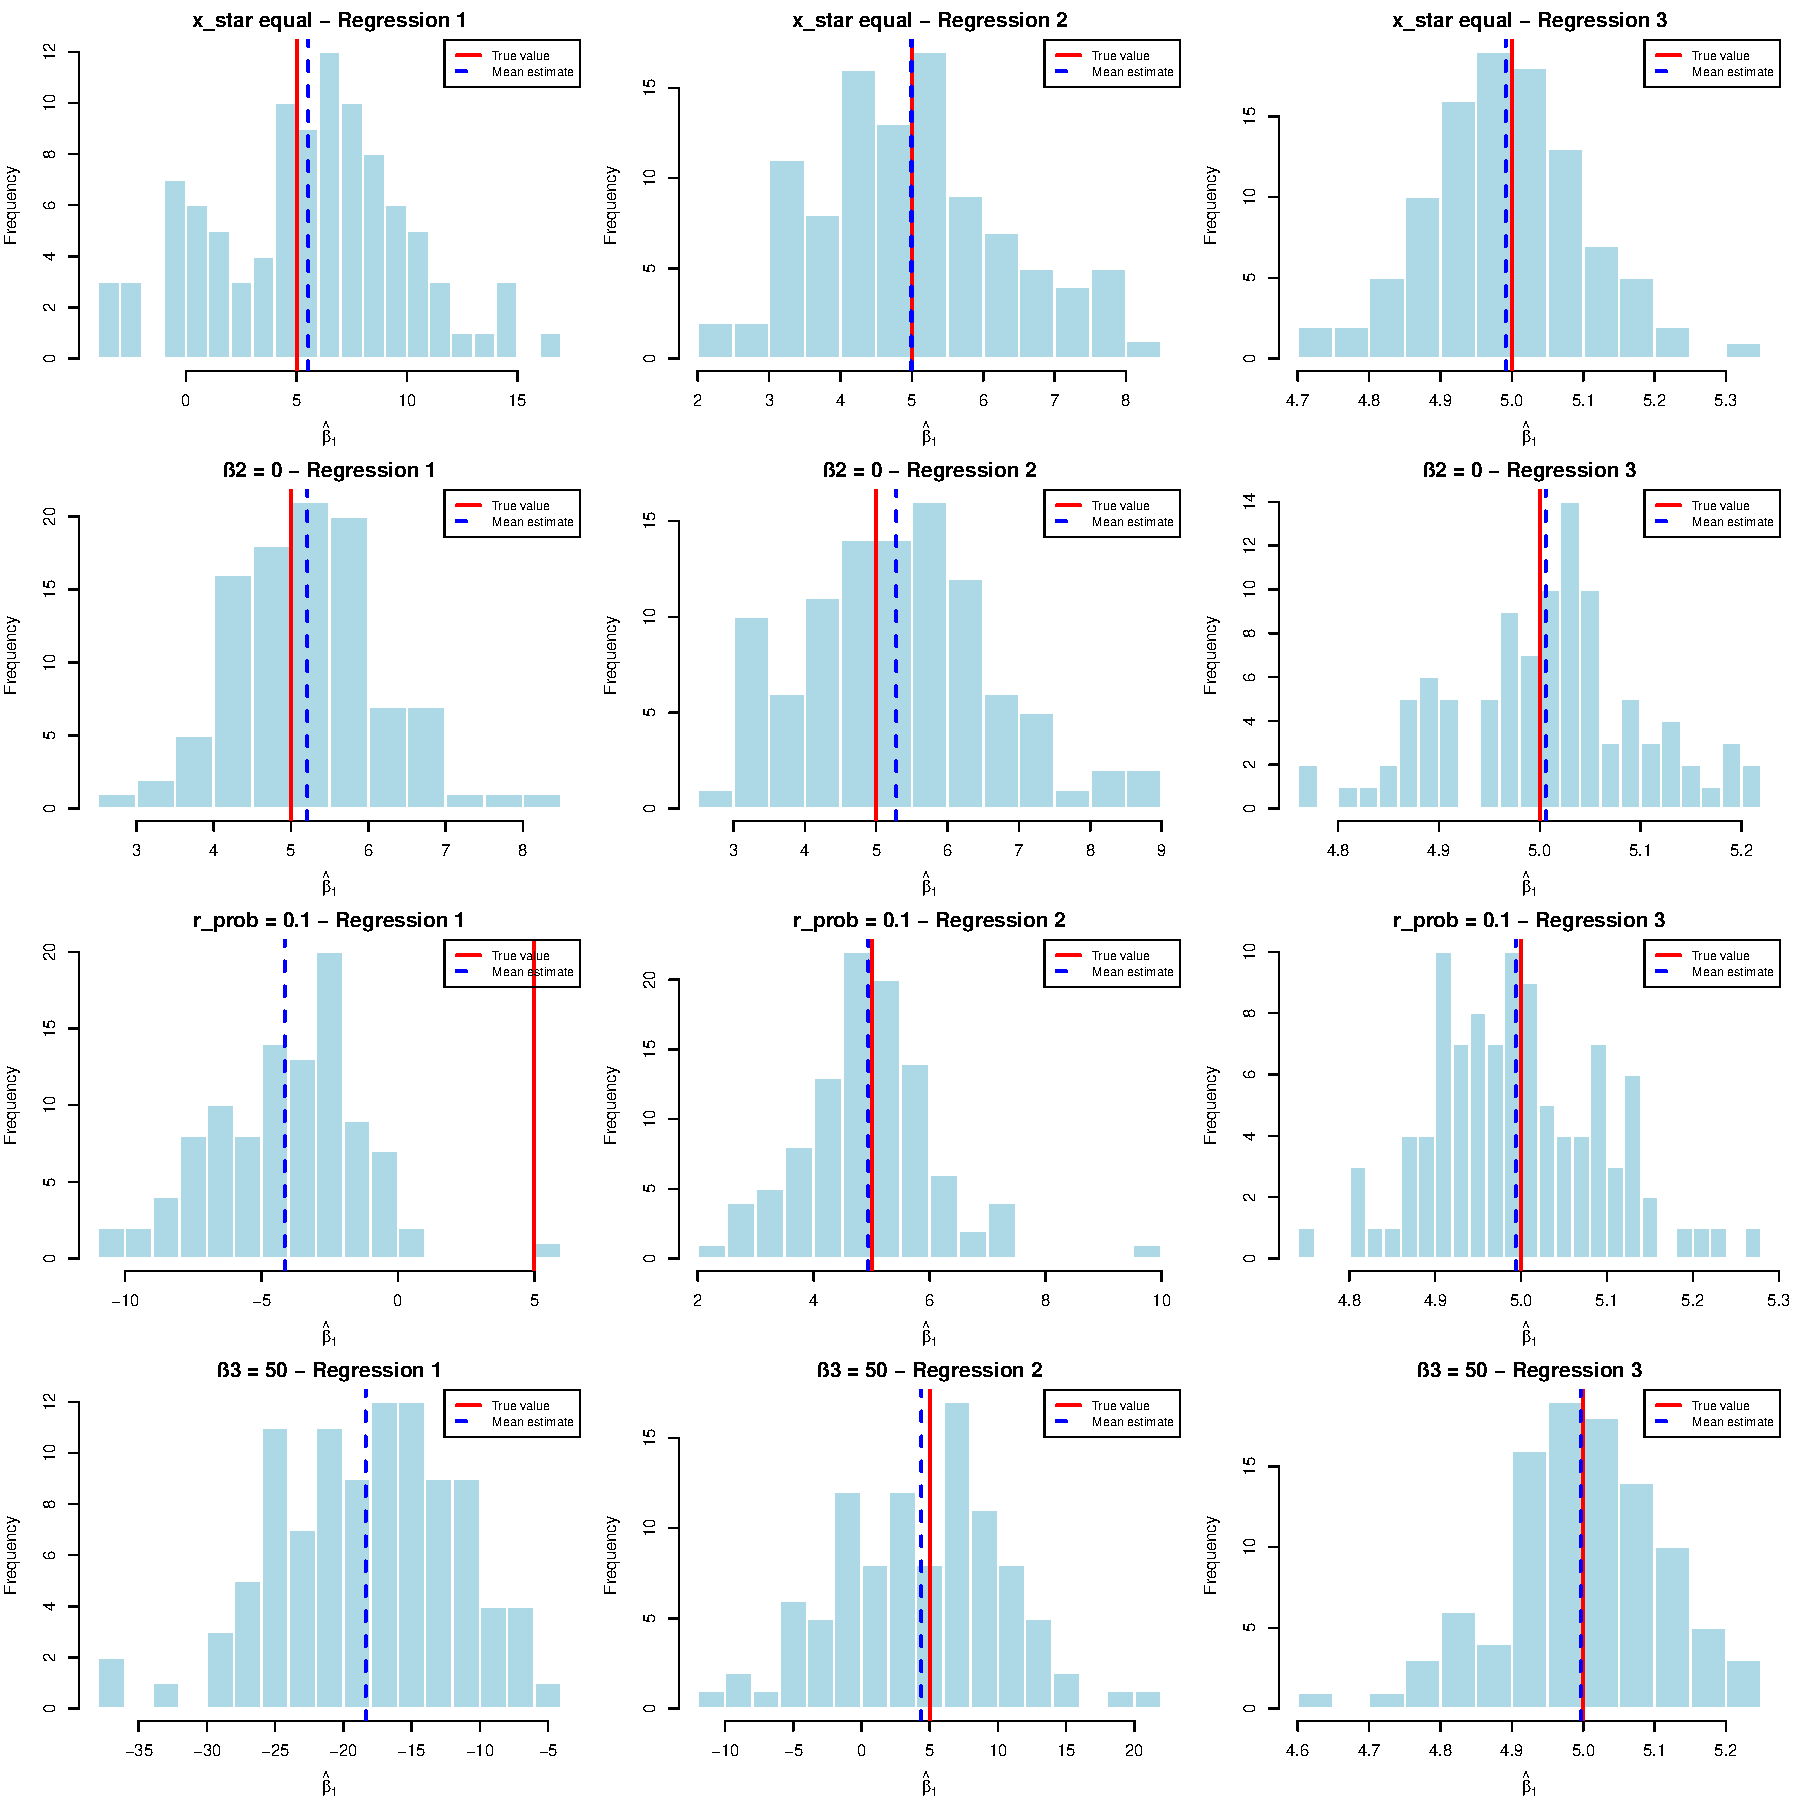
\includegraphics[width=\textwidth]{Q(d).pdf}
\end{figure}


\begin{lstlisting}[language=R]
run_monte_carlo <- function(x_star_equal = FALSE, beta2_zero = FALSE, r_prob = 0.5, beta3_value = 10) {
  M <- 100
  n <- 100

  beta1_estimates <- matrix(NA, nrow = M, ncol = 3)
  colnames(beta1_estimates) <- c("Reg1", "Reg2", "Reg3")
    
  for (m in 1:M) {
    # Generate data according to modified DGP
    u_i <- rnorm(n, mean = 0, sd = sqrt(5))
    g_i <- rgamma(n, shape = 2, scale = 2)
    r_i <- rbinom(n, size = 1, prob = r_prob)
    
    x_star_i <- numeric(n)
    if (x_star_equal) {
      x_star_i <- rgamma(n, shape = 5, scale = 1)
    } else {
      for (i in 1:n) {
        if (r_i[i] == 1) {
          x_star_i[i] <- rgamma(1, shape = 3, scale = 1)
        } else {
          x_star_i[i] <- rgamma(1, shape = 7, scale = 1)
        }
      }
    }

    beta_0 <- 400
    beta_1 <- 5
    beta_2 <- ifels\mathbb{E}[beta2_zero, 0, 200]
    beta_3 <- beta3_value

    y_i <- beta_0 + beta_1 * x_star_i + beta_2 * r_i + beta_3 * g_i + u_i
    
    data <- data.frame(
      y = y_i,
      x_star = x_star_i,
      r = r_i,
      g = g_i
    )
    
    reg1 <- lm(y ~ x_star, data = data)
    reg2 <- lm(y ~ x_star + r, data = data)
    reg3 <- lm(y ~ x_star + r + g, data = data)
    
    beta1_estimates[m, 1] <- coef(reg1)["x_star"]
    beta1_estimates[m, 2] <- coef(reg2)["x_star"]
    beta1_estimates[m, 3] <- coef(reg3)["x_star"]
  }
    
  return(beta1_estimates)
}
  
results_original <- run_monte_carlo()
results_xstar_equal <- run_monte_carlo(x_star_equal = TRUE)
results_beta2_zero <- run_monte_carlo(beta2_zero = TRUE)
results_r_prob_0.1 <- run_monte_carlo(r_prob = 0.1)
results_beta3_50 <- run_monte_carlo(beta3_value = 50)

calc_summary <- function(results, scenario_name) {
  summary_df <- data.frame(
    Scenario = rep(scenario_name, 3),
    Regression = c("Reg1", "Reg2", "Reg3"),
    Mean = colMeans(results),
    SD = apply(results, 2, sd),
    Bias = colMeans(results) - 5
  )
  return(summary_df)
}
  
summary_original <- calc_summary(results_original, "Original DGP")
summary_xstar_equal <- calc_summary(results_xstar_equal, "x_star equal")
summary_beta2_zero <- calc_summary(results_beta2_zero, "β₂ = 0")
summary_r_prob_0.1 <- calc_summary(results_r_prob_0.1, "r_prob = 0.1")
summary_beta3_50 <- calc_summary(results_beta3_50, "β₃ = 50")

all_summaries <- rbind(
  summary_original,
  summary_xstar_equal,
  summary_beta2_zero,
  summary_r_prob_0.1,
  summary_beta3_50
)
  
latex_table_d <- kable(all_summaries, format = "latex", booktabs = TRUE,
                       caption = "Simulation Summary Statistics for Question (d)")
  
output_file_d <- "d.tex"
cat(latex_table_d, file = output_file_d)
cat("\n%% Table saved to ", output_file_d, "\n", sep = "", file = output_file_d, append = TRUE)

scenarios <- list(
  "x_star equal" = results_xstar_equal,
  "β₂ = 0"       = results_beta2_zero,
  "r_prob = 0.1" = results_r_prob_0.1,
  "β₃ = 50"      = results_beta3_50
)

pdf("Q(d).pdf", width = 12, height = 12)
par(mfrow = c(4, 3), mar = c(4, 4, 2, 1))
for (scenario in names(scenarios)) {
  current <- scenarios[[scenario]]
  for (i in 1:3) {
    hist(current[, i],
         main = paste(scenario, "- Regression", i),
         xlab = expression(hat(beta)[1]),
         breaks = 20,
         col = "lightblue",
         border = "white")
    abline(v = 5, col = "red", lwd = 2)
    abline(v = mean(current[, i]), col = "blue", lty = 2, lwd = 2) 
    legend("topright",
           legend = c("True value", "Mean estimate"),
           col = c("red", "blue"),
           lty = c(1, 2),
           lwd = 2,
           cex = 0.8)
  }
}
dev.off()
\end{lstlisting}


% \section{Mathematical Extension: Variance Analysis}

% For completeness, let's also examine the variance of our estimators theoretically:

% For Regression 3 (the correctly specified model), under the classical regression assumptions:
% \[
% \text{Var}(\hat{\beta}_1^{(3)}) = \frac{\sigma^2}{\sum_{i=1}^n \left(x^*_i - \bar{x}^*\right)^2 \cdot \left(1 - R^2_{x^* \sim \text{other regressors}}\right)}
% \]
% Where $\sigma^2$ is the variance of the error term (5 in this case) and $R^2_{x^* \sim \text{other regressors}}$ is the $R^2$ from regressing $x^*_i$ on the other independent variables.

% For Regression 4, including the irrelevant variable $n_i$:
% \[
% \text{Var}(\hat{\beta}_1^{(4)}) \geq \text{Var}(\hat{\beta}_1^{(3)})
% \]
% The inequality is due to the loss of degrees of freedom from estimating an additional parameter.

% For Regression 5, including $b_i$ which is correlated with $x^*_i$:
% \[
% \text{Var}(\hat{\beta}_1^{(5)}) > \text{Var}(\hat{\beta}_1^{(3)})
% \]
% The variance is larger due to multicollinearity, which increases the variance inflation factor (VIF) for $x^*_i$.

% \section{Omitted Variable Bias: Formal Derivation}

% To formalize the omitted variable bias in Regression 1, let's consider the projection of the omitted variables onto $x^*_i$:
% \[
% r_i = \delta_1 + \delta_2 x^*_i + v_i
% \]
% \[
% g_i = \gamma_1 + \gamma_2 x^*_i + w_i
% \]
% where $v_i$ and $w_i$ are the error terms orthogonal to $x^*_i$.

% Substituting these into the true model:
% \[
% y_i = \beta_0 + \beta_1 x^*_i + \beta_2 (\delta_1 + \delta_2 x^*_i + v_i) + \beta_3 (\gamma_1 + \gamma_2 x^*_i + w_i) + u_i
% \]
% Rearranging:
% \[
% y_i = (\beta_0 + \beta_2\delta_1 + \beta_3\gamma_1) + (\beta_1 + \beta_2\delta_2 + \beta_3\gamma_2)x^*_i + (\beta_2v_i + \beta_3w_i + u_i)
% \]
% Therefore, in Regression 1, the expected estimate is:
% \[
% E[\hat{\beta}_1^{(1)}] = \beta_1 + \beta_2\delta_2 + \beta_3\gamma_2
% \]
% where $\delta_2$ is the coefficient from regressing $r_i$ on $x^*_i$, and $\gamma_2$ is the coefficient from regressing $g_i$ on $x^*_i$.

% This formalizes the omitted variable bias as a function of:
% \begin{enumerate}
%     \item The effect of the omitted variables on $y_i$ ($\beta_2$ and $\beta_3$)
%     \item The correlation between the omitted variables and $x^*_i$ ($\delta_2$ and $\gamma_2$)
% \end{enumerate}

% This mathematical derivation explains why we expect systematic biases in the misspecified regressions, and how these biases relate to the underlying parameters of the data generating process.

\end{autosolution}
\end{document}

